\documentclass{bioinfo}
\copyrightyear{2012}
\pubyear{2012}

% amsmath package, useful for mathematical formulas
\usepackage{amsmath}
% amssymb package, useful for mathematical symbols
\usepackage{amssymb}

\usepackage{graphicx}
\usepackage{subfigure} 
% cite package, to clean up citations in the main text. Do not remove.
\usepackage{cite}

\usepackage{url}

\begin{document}
\firstpage{1}

% Title must be 150 characters or less
\title[Tracer 1.6]{Bayesian MCMC diagnostics and summarization using Tracer 1.6}

\author[Rambaut \textit{et~al}]{ Andrew Rambaut\,$^{1}$, Alexei J.~Drummond\,$^{2,3}$, Dong Xie\,$^{2,3}$, Marc A.~Suchard\,$^{4,5,6}$}

\address{
$^{1}$Institute of Evolutionary Biology, University of Edinburgh, Edinburgh, UK\\
$^{2}$Department of Computer Science, University of Auckland, Auckland, NZ\\
$^{3}$Centre for Computational Evolution, University of Auckland, Auckland, NZ\\
$^{4,5}$Departments of Biomathematics and Human Genetics, David Geffen School of Medicine at UCLA, and \\
$^{6}$Department of Biostatistics, UCLA Fielding School of Public Health, University of California, Los Angeles, USA \\
}

\history{Received on XXXXX; revised on XXXXX; accepted on XXXXX}

\editor{Associate Editor: XXXXXXX}

\maketitle


% Please keep the abstract between 250 and 300 words
\begin{abstract}

\section{Motivation:}
Computational evolutionary biology, statistical phylogenetics and coalescent-based population genetics are becoming increasingly central to the analysis and understanding of molecular sequence data. 
\section{Results:}
We describe here a software package, Tracer version 1.6, which ... 
\section{Availability:}
Tracer is open-source under the GNU lesser general public license and available at 
\url{http://beast-mcmc.googlecode.com}  %TODO \url{http://github.com/beast-dev/tracer}
and  \href{http://tree.ed.ac.uk/software/tracer}{\url{http://tree.ed.ac.uk}}.

\section{Contact:} 
\href{a.rambaut@ed.ac.uk}{\url{a.rambaut@ed.ac.uk}}, 
\href{alexei@cs.auckland.ac.nz}{\url{alexei@cs.auckland.ac.nz}}
and 
\href{msuchard@ucla.edu}{\url{msuchard@ucla.edu}}

\end{abstract}

\section*{Introduction}

Blah blah 

\begin{itemize}
\item Importance of posterior summaries (as scientifically relevant marginalization of the full posterior distribution)
\item Full posterior distribution is high-dimensional and (often) difficult to visualize
\item Posterior simulator agnostic -- highly used with \textsc{MrBayes} as well
\end{itemize}

\section*{Design and Implementation}

Blah blah 

New features:
\begin{itemize}
\item Three trace types: real, integer, string
\item Kernel density estimates
\item HME
\item AICM
\end{itemize}

\subsubsection*{Graphical user-interface:}

Tracer can analyse either a single MCMC log or combine the shared traces from multiple logs. Traces panel provides the list of the statistical summary from the sampling parameters' values at all states logged during a MCMC process. 

There are 4 analysis tabs to choose from a selected parameter:

%TODO
Estimates - this shows the mean, stdev, confidence intervals and other statistics about the selected parameter. A frequency distribution will also be plotted.
Density - this shows the Bayesian posterior density plot for the selected parameter.
Joint-Marginal - this only appears if exactly 2 parameters are chosen (hold down shift to select multiple parameters). It then plots one against the other to look at their joint-marginal distribution.
Trace - this shows the trace of the parameter against state or generation number. Use this to check mixing, choose a suitable burn-in and look for trends that might suggest problems with convergence.
Multiple parameters can be selected by holding down the shift key. This will overlay the plots for the different parameters allowing comparisons to be made. You can also select multiple trace files as well to compare different runs. If multiple trace files have the same trace names then a "Combined" trace will automatically appear. This can be selected as well as the individual trace files.

%TODO better figures

\begin{figure}[H]
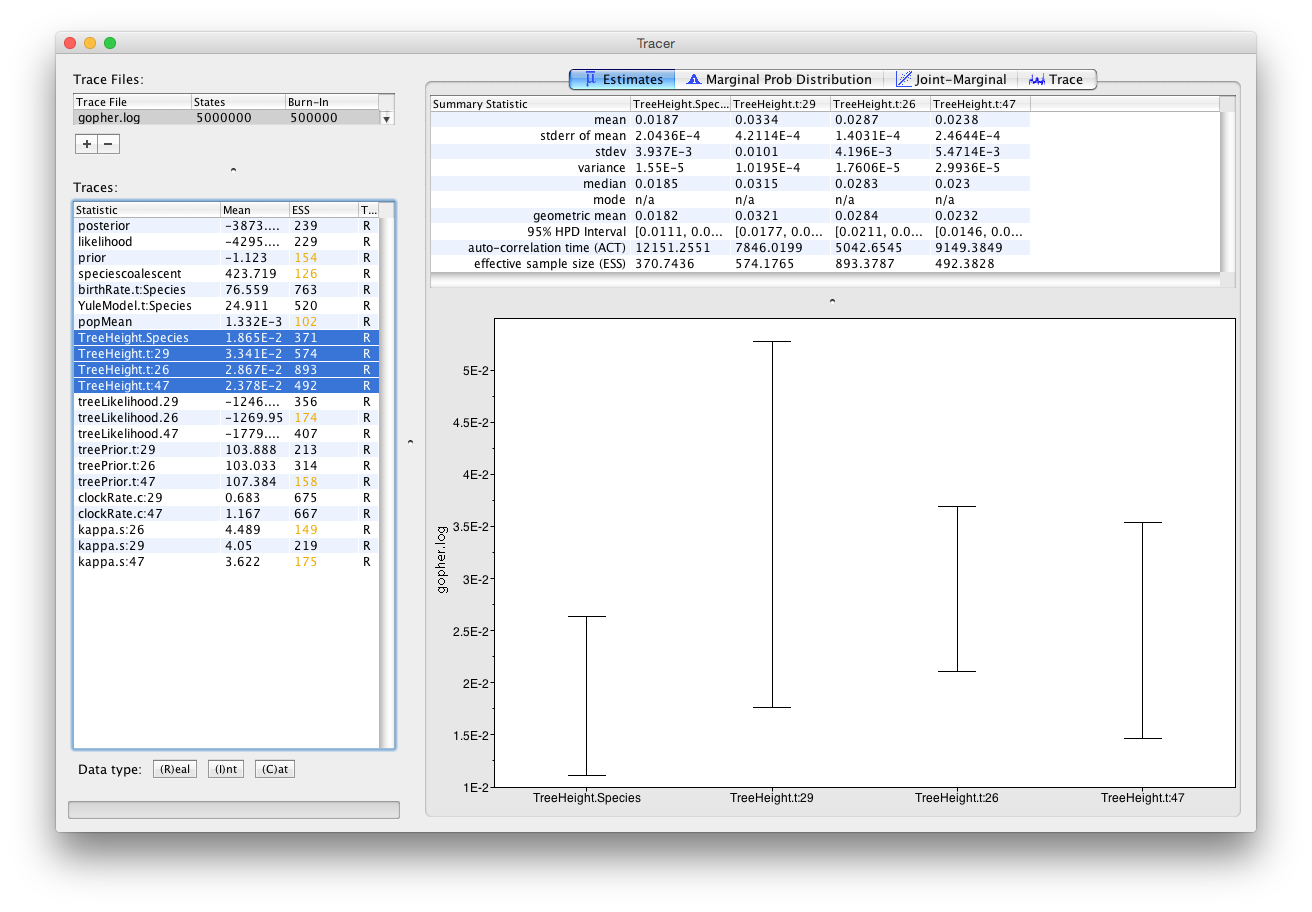
\includegraphics[width=.5\textwidth]{./figures/gopher-log.png}  
\caption{The }
\label{fig:front:page}
\end{figure}

\begin{figure}[H]
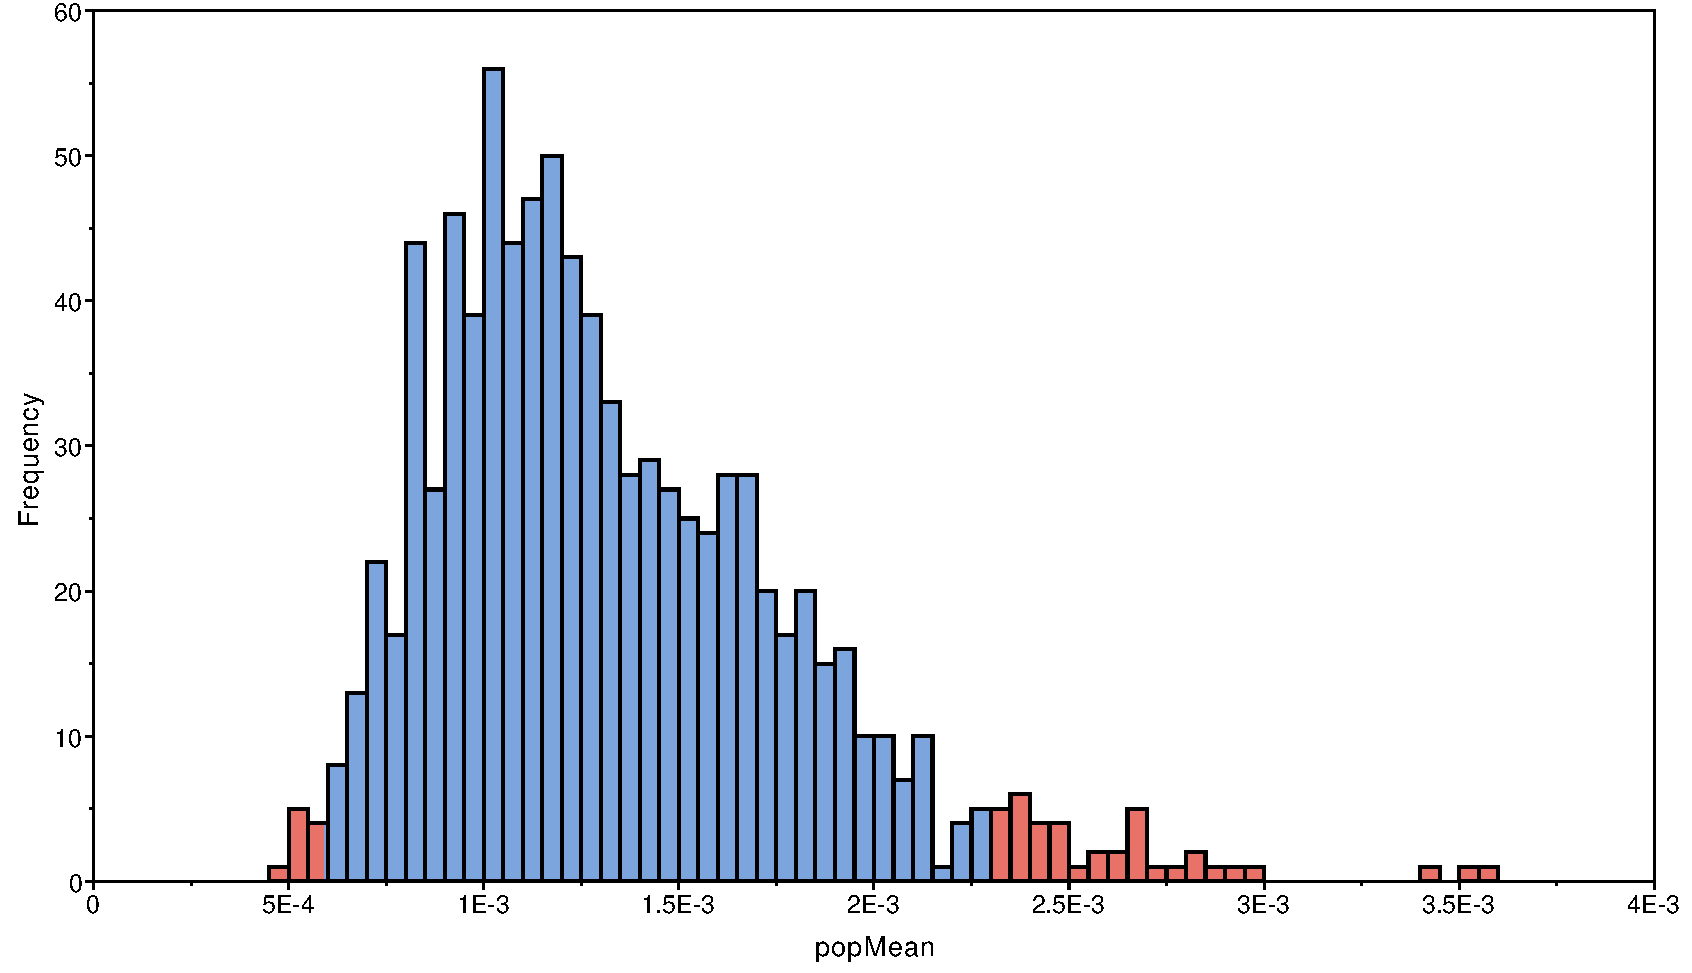
\includegraphics[width=.5\textwidth]{./figures/estimates.pdf}  
\caption{The estimates}
\label{fig:estimates}
\end{figure}

\begin{figure}[H]
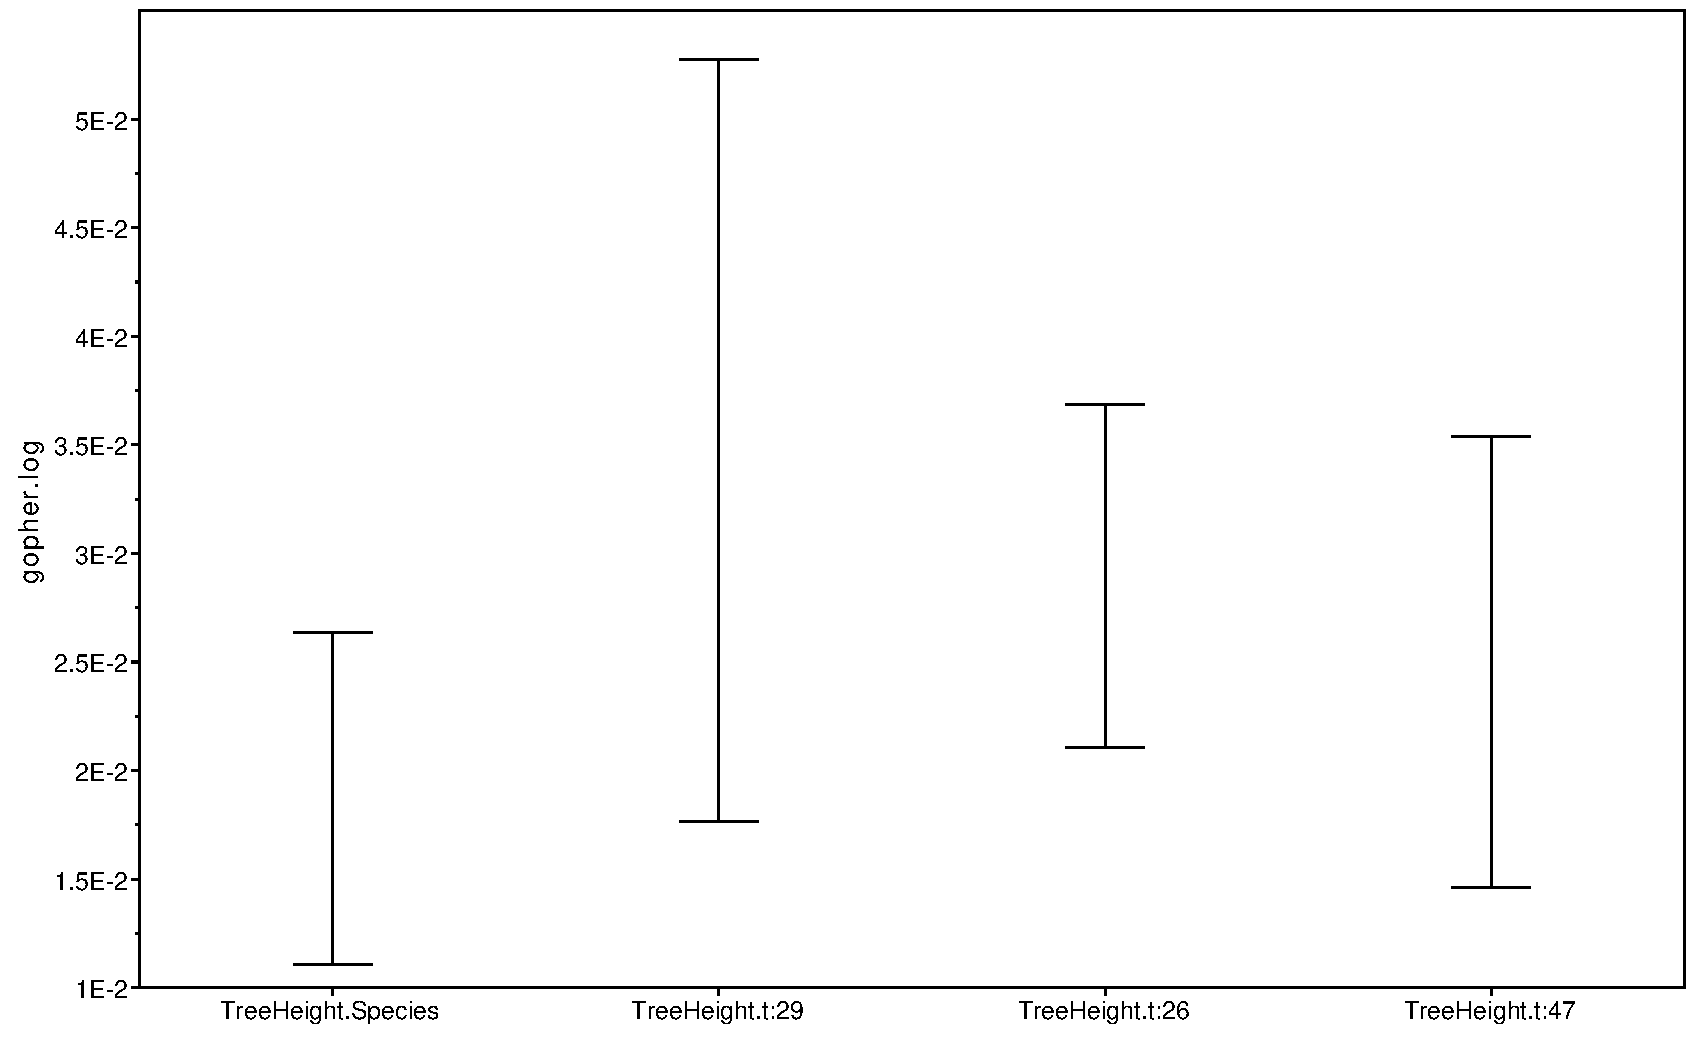
\includegraphics[width=.5\textwidth]{./figures/comp-95HPD.pdf}  
\caption{The comparison of  95\% HPD intervals from multi-trace}
\label{fig:comp95HPD}
\end{figure}

\begin{figure}[H]
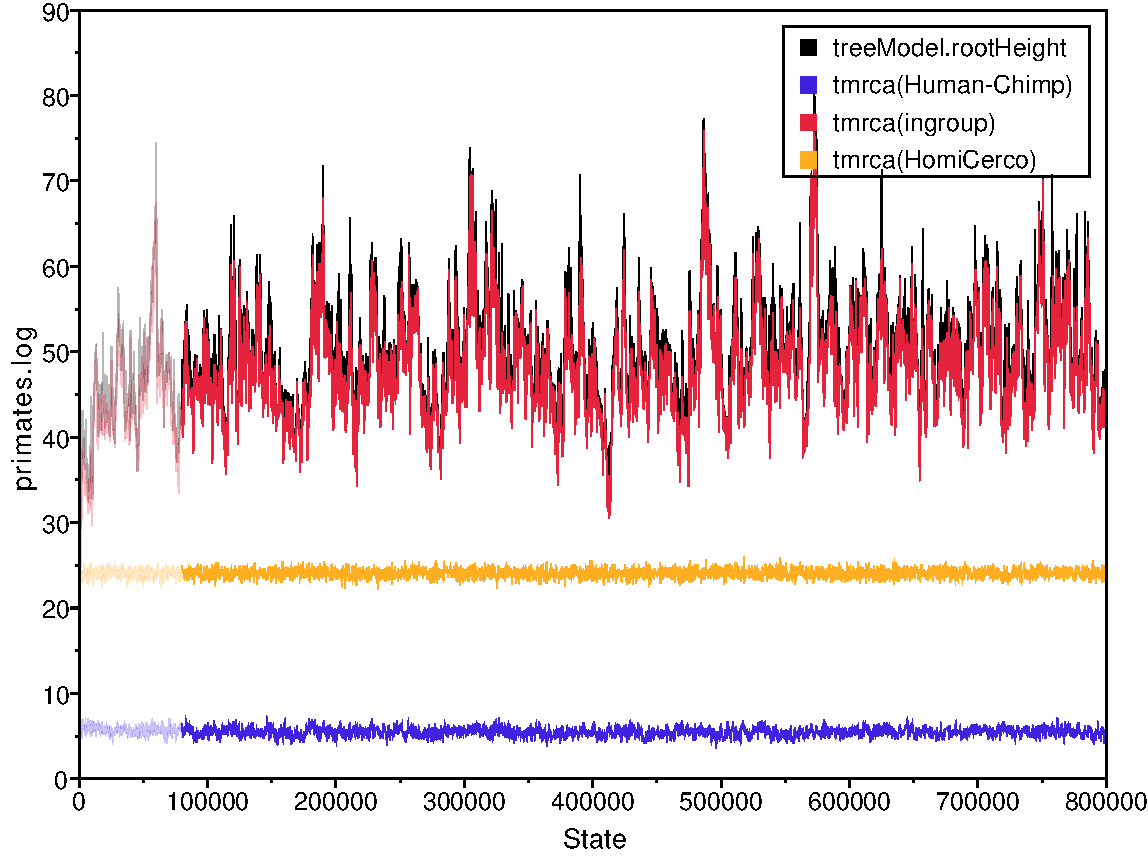
\includegraphics[width=.5\textwidth]{./figures/trace.pdf}  
\caption{The trace}
\label{fig:trace}
\end{figure}


\begin{figure}[H]
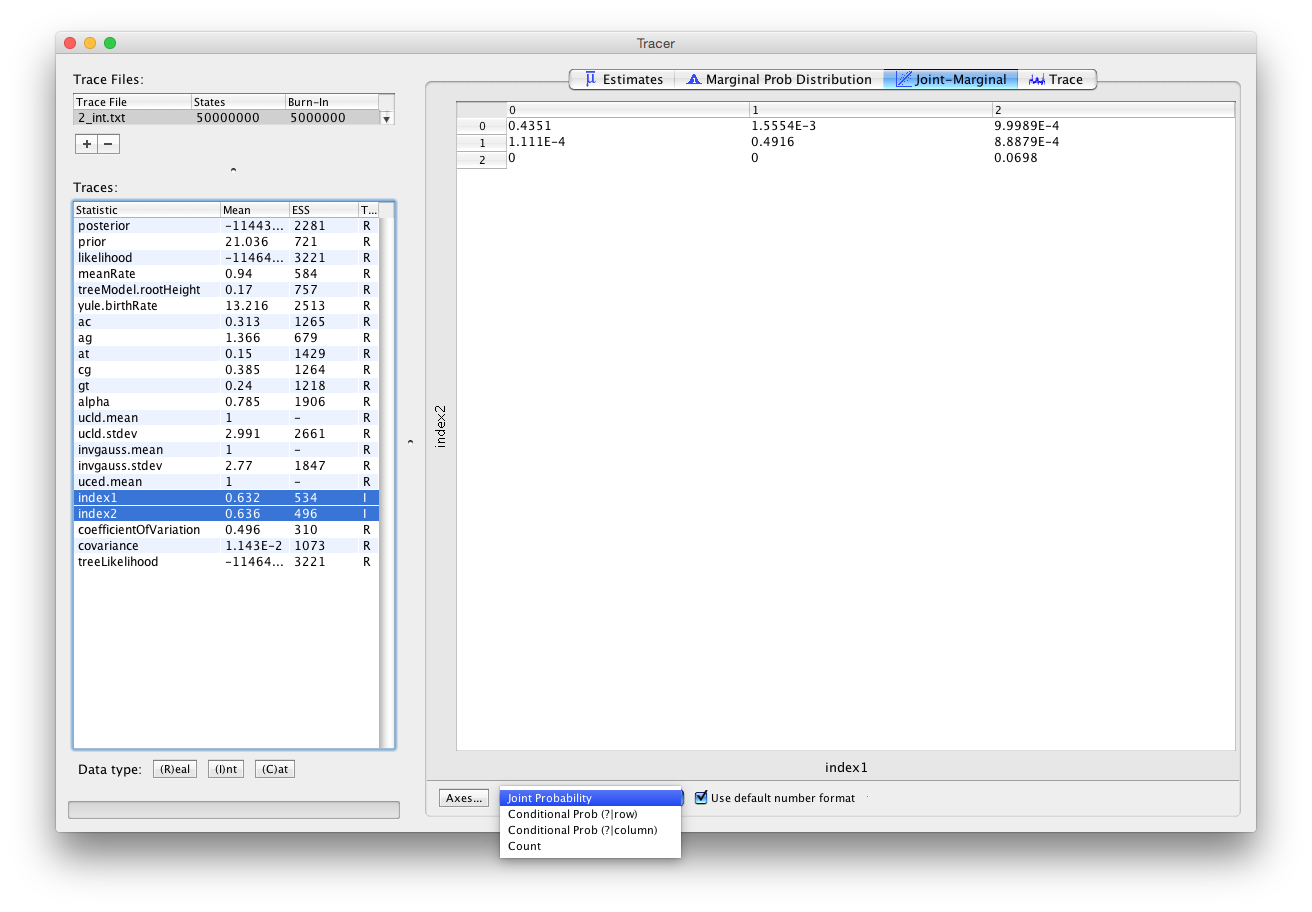
\includegraphics[width=.5\textwidth]{./figures/jointPrInt.png}  
\caption{The Joint probability table of two integer traces}
\label{fig:int:jointpr}
\end{figure}



\subsubsection*{Diagnostics:} Blah blah 

\subsubsection*{Demographic reconstruction:} 

\subsubsection*{Model selection:}


\subsubsection*{Conditional posterior distribution:}

Fairly general solution to looking at conditional posterior distributions;

Specifically, support for BSSVS forms of model averaging, in which some parameters are only in the likelihood when their submodel is "indicated" by some indicator function that is usually a discrete, integer or boolean variable. In that case the posterior of the parameter should not include the states when it was sampled only in the prior because the submodel it belonged to was "turned off". This is relevant for EBSP, Random Local Clocks model, microsatellite model averaging and relaxed clock model averaging methods all from my group in last couple of years. Also relevant for BSSVS in phylogeography as well depending on how the state is logged.


\section*{Example}

Even users of \textsc{MrBayes} and \textsc{RevBayes} find Tracer handy.  

\section*{Availability and Future Directions}

We make the Tracer package available in both executable and source code forms.   Tracer requires Java version 1.5 or greater and executables for Windows, Mac OS and Linux platforms are located at \url{http://beast.bio.ed.ac.uk} which serves as the main page for the package. This page also links to a sizable list of self-contained, step-by-step tutorials covering basic to advance usage of Tracer to summarize posterior distributions of a large set of phylogenetic models simulated using BEAST.  For example, popular tutorials describe how to use Tracer to generate marginal parameter summaries and infer population dynamics trajectories over time.

GoogleCode houses the Tracer's version-controlled source code within \url{http://beast-mcmc.googlecode.com} and links to two GoogleGroup discussion groups related to Tracer.  
The first is the ``beast-users" group (\url{http://groups.google.com/group/beast-users}) with over 1,500 members. 
%At the time of writing, forty-seven developers belong to the ``beast-dev" group that facilitates BEAST development across three continents.

Future development directions for Tracer focus on \ldots


Feature list:
\begin{itemize}
\item KDEs
\item cheap marginal likelihood estimators
\item demographic trajectory reconstruction
\end{itemize}

\section*{Taken from the Tracer website}

Tracer is a program for analysing the trace files generated by Bayesian MCMC runs (that is, the continuous parameter values sampled from the chain). It can be used to analyse runs of BEAST \citep{drummond2007beast,drummond2012bayesian}, BEAST2 \citep{bouckaert2014beast2}, MrBayes \citep{ronquist2012mrbayes}, RevBayes \citep{hohna2016revbayes}, LAMARC \citep{kuhner2006lamarc}, Migrate \citep{beerli2006comparison} and possibly other MCMC programs.

Although Tracer can be used with programs other than BEAST, users may find it useful to join the BEAST users mailing list. This is used to announce new versions and advise users about bugs and problems.

You can join the mailing list here:
http://groups.google.com/group/beast-users

The website for BEAST (and Tracer) is here:
http://beast.bio.ed.ac.uk/

At present there is no detailed manual for this application, you will simply have to play around and see what happens. Basically you can select the trace file in the top left of the window, the individual parameter in the bottom left and the analysis appears on the right.

There are 4 analysis tabs to choose from:

Estimates - this shows the mean, stdev, confidence intervals and other statistics about the selected parameter. A frequency distribution will also be plotted.
Density - this shows the Bayesian posterior density plot for the selected parameter.
Joint-Marginal - this only appears if exactly 2 parameters are chosen (hold down shift to select multiple parameters). It then plots one against the other to look at their joint-marginal distribution.
Trace - this shows the trace of the parameter against state or generation number. Use this to check mixing, choose a suitable burn-in and look for trends that might suggest problems with convergence.
Multiple parameters can be selected by holding down the shift key. This will overlay the plots for the different parameters allowing comparisons to be made. You can also select multiple trace files as well to compare different runs. If multiple trace files have the same trace names then a "Combined" trace will automatically appear. This can be selected as well as the individual trace files.

You can also select the "Demographic Analysis" from the Analysis menu - This plots the distribution of demographic population sizes over time for a number of models (constant size, exponential growth \& logistic growth) that are available in BEAST. This involves you selecting the traces for each parameter of the model. You should only select the model that was actually run under BEAST (e.g., if you ran an exponential growth model, you shouldn't plot the constant population size model).

The "Analysis" menu also contains options for performing Bayesian Skyline reconstructions and for calculating Bayes Factors between runs.

The "Print" function in the "File" menu will print the current graph or table and the "Export Data" function can be used to export the data from the plots for use in another graphic package.

To export the currently displayed graphic use the "Export PDF" function in the "File" menu.



\section*{Acknowledgments}

We thank the National Evolutionary Synthesis Center (NESCent) for sponsoring a working group (Software for Bayesian Evolutionary Analysis) that facilitated the development of Tracer version 1.6. 
This work was supported in part by funding from the Marsden Trust, NSF (DMS 0856099), NIH (R01 GM086887, R01 HG006139), The Royal Society of London, BBSRC (BB/H011285/1) and the Wellcome Trust (WT092807MA).

%\section*{References}
% The bibtex filename
\bibliographystyle{natbib}
\bibliography{tracer16}

\end{document}

